\makeatletter
\providecommand*{\input@path}{}
\g@addto@macro\input@path{{style/}}
\makeatother

\documentclass[a4paper,11pt,oneside]{kth-mag}

% Formatting packages
\usepackage[T1]{fontenc}
\usepackage{textcomp}
\usepackage{lmodern}
\usepackage[utf8]{inputenc}
\usepackage[english, swedish]{babel}
\usepackage{modifications}
\usepackage[final]{pdfpages}

% packages for tables
\usepackage{booktabs}
\usepackage{longtable}

% tikz
\usepackage{tikz}
\usetikzlibrary{bayesnet, shapes.geometric, arrows, shadows, positioning, decorations.pathreplacing,angles,quotes, trees}
% define annotated cube
\tikzset{
  annotated cuboid/.pic={
    \tikzset{%
      every edge quotes/.append style={midway, auto},
      /cuboid/.cd,
      #1
    }
    \draw [every edge/.append style={pic actions, densely dashed, opacity=.5}, pic actions]
    (0,0,0) coordinate (o) -- ++(-\cubescale*\cubex,0,0) coordinate (a) -- ++(0,-\cubescale*\cubey,0) coordinate (b) edge coordinate [pos=1] (g) ++(0,0,-\cubescale*\cubez)  -- ++(\cubescale*\cubex,0,0) coordinate (c) -- cycle
    (o) -- ++(0,0,-\cubescale*\cubez) coordinate (d) -- ++(0,-\cubescale*\cubey,0) coordinate (e) edge (g) -- (c) -- cycle
    (o) -- (a) -- ++(0,0,-\cubescale*\cubez) coordinate (f) edge (g) -- (d) -- cycle;
    \path [every edge/.append style={pic actions, |-|}]
    (b) +(0,-5pt) coordinate (b1) edge ["\cubex \cubeunits"'] (b1 -| c)
    (b) +(-5pt,0) coordinate (b2) edge ["\cubey \cubeunits"] (b2 |- a)
    (c) +(3.5pt,-3.5pt) coordinate (c2) edge ["\cubez \cubeunits"'] ([xshift=3.5pt,yshift=-3.5pt]e)
    ;
  },
  /cuboid/.search also={/tikz},
  /cuboid/.cd,
  width/.store in=\cubex,
  height/.store in=\cubey,
  depth/.store in=\cubez,
  units/.store in=\cubeunits,
  scale/.store in=\cubescale,
  width=10,
  height=10,
  depth=10,
  units=cm,
  scale=.1,
}
% define document shape
\makeatletter
\pgfdeclareshape{document}{
\inheritsavedanchors[from=rectangle] % this is nearly a rectangle
\inheritanchorborder[from=rectangle]
\inheritanchor[from=rectangle]{center}
\inheritanchor[from=rectangle]{north}
\inheritanchor[from=rectangle]{south}
\inheritanchor[from=rectangle]{west}
\inheritanchor[from=rectangle]{east}
% ... and possibly more
\backgroundpath{% this is new
% store lower right in xa/ya and upper right in xb/yb
\southwest \pgf@xa=\pgf@x \pgf@ya=\pgf@y
\northeast \pgf@xb=\pgf@x \pgf@yb=\pgf@y
% compute corner of ‘‘flipped page’’
\pgf@xc=\pgf@xb \advance\pgf@xc by-5pt % this should be a parameter
\pgf@yc=\pgf@yb \advance\pgf@yc by-5pt
% construct main path
\pgfpathmoveto{\pgfpoint{\pgf@xa}{\pgf@ya}}
\pgfpathlineto{\pgfpoint{\pgf@xa}{\pgf@yb}}
\pgfpathlineto{\pgfpoint{\pgf@xc}{\pgf@yb}}
\pgfpathlineto{\pgfpoint{\pgf@xb}{\pgf@yc}}
 \pgfpathlineto{\pgfpoint{\pgf@xb}{\pgf@ya}}
\pgfpathclose
% add little corner
\pgfpathmoveto{\pgfpoint{\pgf@xc}{\pgf@yb}}
\pgfpathlineto{\pgfpoint{\pgf@xc}{\pgf@yc}}
\pgfpathlineto{\pgfpoint{\pgf@xb}{\pgf@yc}}
\pgfpathlineto{\pgfpoint{\pgf@xc}{\pgf@yc}}
}
}
\makeatother

%fix Reference URLs
\usepackage[hyphens]{url}
\usepackage[hidelinks]{hyperref}
\hypersetup{breaklinks=true}
\urlstyle{same}


% other packages
\usepackage{pgfplots}
\usepackage{pgfplotstable}
\usepackage{amsmath}
\usepackage{amssymb}
\usepackage{multirow}
\usepackage{float}
\usepackage{csquotes}
\usepackage{amsmath}
\usepackage{listings}
\usepackage[caption=false]{subfig}
\usepackage[flushleft]{threeparttable}
\usepackage{placeins}


%define colors
\definecolor{mygreen}{RGB}{27,158,119}
\definecolor{myyellow}{RGB}{255,237,160}
\definecolor{myorange}{RGB}{254,178,76}
\definecolor{myred}{RGB}{240,59,32}
\definecolor{mylightpurple}{RGB}{178,171,210}
\definecolor{mypurple}{RGB}{94,60,153}
\definecolor{mylightgreen}{RGB}{153,216,201}
\definecolor{mylightblue}{RGB}{43,131,186}



%PGFplot stuff
\pgfplotsset{compat = 1.10}
\pgfplotsset{
    discard if not/.style 2 args={
        x filter/.code={
            \edef\tempa{\thisrow{#1}}
            \edef\tempb{#2}
            \ifx\tempa\tempb
            \else
                \def\pgfmathresult{inf}
            \fi
        }
    }
}
\usepgfplotslibrary{statistics}



% Defined math operators
\DeclareMathOperator*{\argmin}{arg\,min}
\DeclareMathOperator*{\argmax}{arg\,max}

% glossaries package and necessary commands to resolve conflicts
\let\printglossary\relax
\let\theglossary\relax
\let\endtheglossary\relax
\selectlanguage{english}
\usepackage[
nonumberlist,
	acronym,			
	shortcuts,% acronym shortcuts
]{glossaries}
%\makenoidxglossaries



%%%%%%%%%%%%%%%%%%%%%%%%%%%%%%%%%%%%%%%%%%%%%%%%%%%%%%%%%%%%%%%%%%%%%%%%%%%%%%

\title{Ethics and Implications of the Free-to-Play Business Model in the Game Industry}



% TODO: Add swedish title
\foreigntitle{}
\author{Davide Anghileri}
\date{\today}
\blurb{EIT Digital Data Science \\ Minor's Thesis\\ KTH - Royal Institute of Technology\\ Supervisor: Bo Karlson\\
} 

\trita{}




%%%%%%%%%%%%%%%%%%%%%%BIB SETTINGS %%%%%%%%%%%%%%%%%%%%%%%%%%%%%%%%%%%

\usepackage[style=ieee, backend=biber, sorting=none, isbn=false, doi=false, url=false, maxcitenames=2, mincitenames=1, maxbibnames=8]{biblatex}
\setlength{\bibitemsep}{1em}     % Abstand zwischen den Literaturangaben
\setlength{\bibhang}{2em}        % Einzug nach jeweils erster Zeile
\usepackage[a4paper]{geometry}
\toks0\expandafter{\biburlsetup} % Settings to remove extra spaces in URLs
\edef\biburlsetup{\the\toks0 \Urlmuskip =0mu\relax}
\newcommand{\code}[1]{\texttt{#1}}

\DeclareBibliographyDriver{online}{%this defines what will be printed in the bibliography for entries of type 'online'
  \usebibmacro{author}
  \setunit{\addcomma\addspace}%comma+space
  \usebibmacro{title}
  \usebibmacro{note+pages}
  \setunit{\addperiod\addspace}%Period+space after 'Note' field
  \usebibmacro{url+urldate}
  \usebibmacro{finentry}}


\bibliography{./biblio.bib}

\AtEveryBibitem{%
  \ifentrytype{book}
    {\clearfield{url}
   \clearfield{editor}}
    {}%
}

\AtEveryBibitem{%
  \ifentrytype{incollection}
    {\clearfield{url}}
    {}%
}

\AtEveryBibitem{%
  \ifentrytype{inproceedings}
    {\clearfield{eventtitle}}
    {}%
}

\AtEveryBibitem{%
    \clearfield{volume}%
}

\AtEveryBibitem{%
  \clearfield{note}%
}
 


%%%%%%%%%%%%%%%%%%%%%% END BIB SETTINGS %%%%%%%%%%%%%%%%%%%%%%%%%%%%%%


\begin{document}

%REMOVE COMMENT 
\includepdf[noautoscale,pages=1]{kth-cover}

\frontmatter
\pagestyle{empty}
\removepagenumbers
\maketitle
\clearpage
\selectlanguage{english}
% Abstracts 
%REMOVE COMMENT \begin{abstract}





\end{abstract}

\clearpage




\begin{foreignabstract}{swedish}

\end{foreignabstract}
%REMOVE COMMENT \chapter*{Acknowledgments}



\vspace{1.0cm}

\noindent
Stockholm, \today

\noindent
\textit{Davide Anghileri}

\clearpage
\tableofcontents*
\clearpage
%\printnoidxglossaries 
% \printnoidxglossary[type=\acronymtype]
\mainmatter
\pagestyle{newchap}
\chapter{Introduction}
Within the recent years, we have seen an incredible growth in the gaming industry. Newzoo, a leading provider of games market intelligent, reported that “the gaming industry is growing faster than expected, up 10.7\% to \$116 billion 2017” \cite{_newzoo:_????}. As visible in Figure \ref{fig:newzoo2}, half of the global game market is represented by the mobile industry, including tablets and smartphones and the future perspectives show a continuous growth at an annual rate of 8.2\% up to 2020. 
\begin{figure}
    \centering
    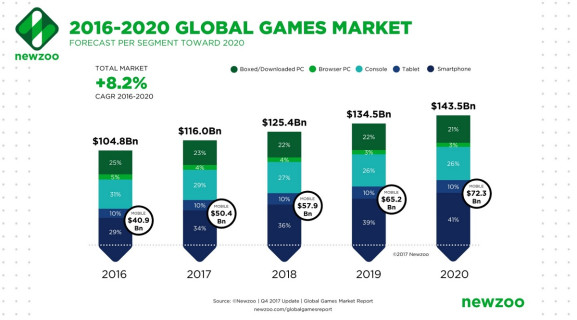
\includegraphics{masters-thesis-master/masters-thesis/contents/01_introduction/newzoo-2.jpg}
    \caption{Trend of the mobile game industry from 2016 to 2020. Image from \cite{_newzoo:_????} }
    \label{fig:newzoo2}
\end{figure}
Furthermore, as showed in Figure \ref{fig:newzoo3} the mobile market segment is growing faster compared to the other segments in the game industry, with a year on year growth rate of 23.3\% in 2017.
\begin{figure}
    \centering
    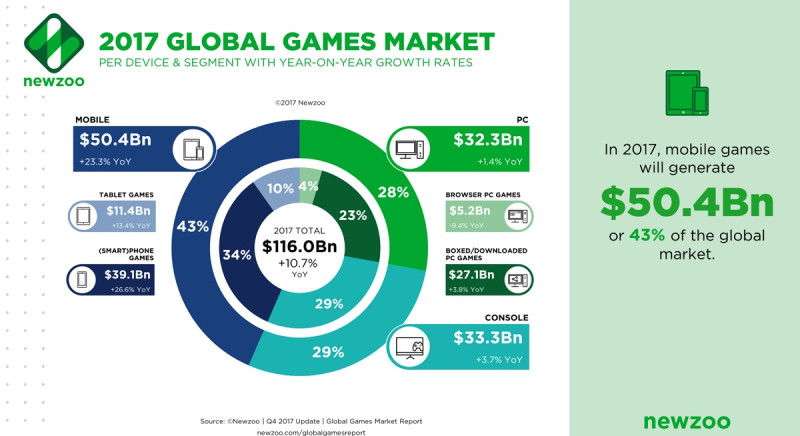
\includegraphics[width=\textwidth]{masters-thesis-master/masters-thesis/contents/01_introduction/newzoo-3.jpg}
    \caption{Per device and segment global games market and year-to-year growth rates . Image from \cite{_newzoo:_????} }
    \label{fig:newzoo3}
\end{figure}
Everyday more and more people use their tablet or smartphone to play video games and a recent report on Verto Analytics \cite{_report:_2016} showed that gamers play an average of 24 minutes each day. These incredible numbers motivate why it is important to deeper understand what is going on in this sector and which implications are emerging. First of all, a key factor in this growth is the cheaper and higher quality technology as well as the possibility of accessing Internet almost everywhere, enabling the development of more engaging games. As an example, nowadays is easy to play a game online, together with a friend, sharing achievements, competing in a leader-board or exchanging virtual gifts. But just like the technologies and the way we play video games has changed, also the way game companies make money from video games has changed too. 

\section{From Pay-to-Play to Free-to-Play Business Model}
A current trend is the shift from the traditional Pay-to-Play (P2P) business model to the Free-to-Play (F2P) or “freemium” business model. The F2P model allows users to acquire and play a game free of charge and at the same time, encourages them to pay for in game additional content  with different purpose, e.g. unlocking content, avoiding ads, buying boosters, etc. More than that, it allows game companies to increase the popularity of a game and to collect revenues later on. On the contrary, the P2P business model describes those game where the user must pay before obtaining the game and then the game content is free. Previously, the players paid once and then they played as mush as they wanted. Now,  the potential profit of a single game is theoretically infinite dollars. This shift is demonstrated by the tremendous success of many F2P games like Candy Crush Saga (King.com 2012), Clash Royal (Supercell 2016) or Hearthstone (Blizzard Entertainment 2014). Even if there are also some example of profitable P2P games like Minecraft (Microsoft Studios 2011), the evidence of this shift is indicated by the fact that Apple Store is dominated by apps that use a F2P business model. The free-to-play business model dates back to  1999 when it was first used in the Nexon's QuizQuiz game, made by Lee Seungchan. However is only in the last decade that it has become the leading way of monetizing games.

To be precise, also slightly different business models are possible. World of Warcraft (WoW), a multiplayer online game (Blizzard Entertainment 2004), is an example of a game where the user needs to pay to maintain an active account. However, since the player has no choice and he must pay if wants to play the game, we will consider it as a P2P game. Finally, demos can be considered as F2P games since the player can try the game for free and decides later if buying or not the game. 

A key factor in favour of the F2P business model is the low or almost zero barriers for new users, since the game requires only a smartphone and a good enough internet connection to be downloaded. This allows F2P games to acquire large scale visibility and a bigger user base. Another important aspect that has favored this shift is the change in the market user base. Nowadays, gaming is a mass market and most of the published games are casual games, addressed to everyone. 

In a sense, a F2P game can be seen as a service rather than as a physical product. This changes the way the game is created and maintained with implications on both players and game companies. In literature, this phenomena is called \textit{servitization}.

\section{Servitization}

The word "servitization" dates back to the 80s and it was first used in \cite{vandermerwe_servitization_1988}. It was defined as "adding value by adding services". However, is only recently that this word started to attract interest and attention both in the literature and in the company environments. Firms started to see marketing opportunity and business growth by the adoption of service strategies.
Servitization is a transformation journey that involves companies that decide to shift from selling product, in our case a P2P game, to selling product-service systems, in our case a F2P service-game. A service-product system consist of a mix of goods and services that deliver value to the final customer. Being able to successfully face this shift, requires good capabilities, strong strategies and imply significant changes.
Rolls-Royce is a concrete example of a company that successfully adopted the servitization business model selling "power-by-the-hour". Instead of selling aircraft engines they switched and started to sell the "power of the engines". The customers can rent the engines and Rolls-Royce provide support and additional services, including maintenance. 
A similar transformation is happening in the game industry as well thanks to the adoption of the F2P business model. The core value that game companies deliver is no more the product itself, the game, but the whole system of services, support, community, merchandising and activities around it.
In this research we are interested into the impacts and consequences of this business strategy in the game industry.
\textcite{zhang_challenges_2017} identified five different challenges: organisational structure, business model, development process, customer management, and risk management. 
Focusing on the game industry, we are interested into analyzing how servitization is affecting these five aspect with a strong focus on ethical considerations.




\section{Research Question}
Monetization strategies are various and complex and in the literature there are interesting analysis of how they work and why people pay for in game content \cite{hamari_why_2015} both from a financial and a psychological perspective. However, the F2P business model creates some implications that are analyzed in this research. While monetization strategies \cite{holin_lin_cash_2011, park_exploring_2011, davidovici-nora_paid_2014} and games \cite{zagal_dark_2013} have been widely investigated in the literature, there is a knowledge gap on the impact and effects of this new business model both from the user perspective and the company perspective. As a consequence, the research question to be analyzed is:
\begin{center}
        \textit{ Which are the implications for players and game designers of the shifting from pay-to-play to free-to-play business model in the game industry?
}
\end{center}


\section{Outline}
The rest of this minor thesis is structured as follows:
Chapter \ref{chap:background} presents a discussion about the implications that this shift has on the players. Chapter \ref{chap:results} describes the implications from the perspective of game companies and game designers. Finally, conclusions are reported in Chapter \ref{chap:conclusions}.

\chapter{Player Implications}
\label{chap:background}
\section{Pay-to-Win}
The F2P business model arises many implications on players and in this chapter we discuss and analyze the most relevant.
A first implication is when a player can purchase game content that allows him to gain a significant and unfair advantage over the non paying players. This is informally called "Pay-to-Win" effect. Paywalls, is the term used to describe the points where, if a player does not pay, the advancement in the game is stopped. It happens especially in multiplayer games and can create frustration or disappointment in the non paying players leading them to abandon the game or turn into paying users. Pay-to-Win games are usually criticized both from players but also from game designer. They usually connect this phenomena to an unfair and not fun game \cite{alha_free--play_2014}. 
A common approach to avoid that in-game purchases affects gameplay is to allow players to buy only "cosmetic" items e.g. skins, avatars, emotes, themes. League of Legends (Riot Games 2009) and Dota 2 (Valve Corporation 2013) are only two examples of games that adopt this approach. Other games, like Clash of Clans (Supercell 2012), even if allows non-paying players to acquire and collect any game content, due to time constraints, becomes impracticable to play the game competitively without paying. A common justification of Pay-to-Win publishers is: “anything you can buy with real money, can be obtained by simply playing the game”, but even if this is usually true, the time or effort required by the player to obtain the same content of a paying user is usually unfeasible. Nevertheless, the opinion of the players can sometimes make the difference. As an example, when the beta of the game Star Wars Battlefront (EA DICE 2017) was released, the fans strongly protested about the new game progression system and convinced the company to entirely remove the microtransactions system from the game just few hours before its worldwide launch \cite{kain_ea_????, tassi_ea_????}.
\section{Whales} 
From an ethical point of view, one of the most important and critical phenomena that the F2P business model has generated, is the so called "Whale". This concept refers to those people who spend lot of money with in-app purchases and microtransactions. The term was first used by salesmen referring to big clients and also by casinos to refer to big spenders. A statistic reported on Forbes \cite{tassi_why_????}, showed that only 0.15 percent of players contribute to 50 percent of the revenues. Similarly, the website \textit{Tapjoy} \cite{_infographic:_????} has analyzed the habits of players of F2P games, and calculated that whales make on average 7.4 in-app purchases per month, for a median average revenue per paying user (ARPPU) of 335 \$. To give a concrete example of this phenomena, in 2012, at the Game Developers Conference, the 5th Planet chief executive Robert Winkler, announced \cite{_what_2013} that in the game Clash of the Dragons, 40 percent of revenues came only from 2 percent of the gamers spending 1.000 \$ or more. But who are the whales? A demographic report \cite{good_who_????} showed that two third of the whales are male with an average age of 30 years old. Furthermore, it analyzed the time spent on a game and emerged that the time spent by whales is grather by a factor of three compared to other players. Finally, they showed that smartphones and tablet generate almost half of the whales in the whole game industry. For a deeper analysis on whales behaviour we refer to \cite{_how_2015}. 

In the app store there are games that are clearly developed with the idea of whales in mind. Whenever we find a game which makes virtually impossible to keep on playing without paying is a clear sign that game designers want to make us spend. We need to remember that even video games are an industry and as any other industry the main objective is to make money. However, there are some peculiarities that makes game profits morally questionable. There is no clear amount of money to distinguish whales from normal paying players but the term usually refers to people who spends hundreds or thousands of dollars with in-game purchases. Even if everyone has the right to do whatever they wants with their money, the average whale is not a rich person with lot of money to spend but he is usually a common person that decides to spend most of his money in a specific game. Also, the marketing strategy of trying to take as much money as possible from a small subset of players, in order to cover for the non paying players, creates some ethical considerations. 

Finally, we need to consider that buying game content is not the same as buying a normal product. When a player buys game content, he does not own the content, he only own the right to see it. He can not trade, re-sell, or donate it. Furthermore, the purchase is available till the game is alive. But what becomes of all the purchases if the game is shut down?  

\section{Addiction}
Also, as other forms of entertainment, games can create addiction. Especially if we consider F2P games, created with the goal of retaining users as long as possible, exploiting those human mechanism weaknesses which can lead to addiction. Games addiction is a serious problem that can involve people of different ages and can determine social isolation, low imagination, mood alterations and exclusion of real life events in favour of virtual achievements or rewards. Many games rely on a cycle of activities that the player has to continue to perform and that is called "compulsion loop". A game reward can generate the neurological reaction of releasing dopamine, making the player feel satisfied. A very similar reaction occurs with gambling addiction. An even more serious problem happen when a player finds these satisfactions only in a virtual game and do not feel the same emotions in the real world. We need to say that encouraging a deeper and deeper engagement is not only a problem of games but concern every entertainment activity like watching movies or others forms of media.

A peculiarity is that, if we look at the top highest grossing mobile games we can see that most of them offers poker, slot dice games or others games like in a real casino. Is quite obvious to think that they are making money from gambling, indeed, they are just games. Despite the fact that they offer in app purchases to fund turns, they do not offer any real money pay-out. Players can play these "games" just for fun. Double Down Casino (Double Down Interactive 2012) is an example of such a game and it offers prices only with virtual currency. People play only for fun or competition with friends. 

The presence of virtual currency in most of the F2P games that are available today, from a psychological point of view, creates an issue. For some players, earning, managing and spending virtual money, are carried out with the same criteria and feelings we use for real money. Prof. Mark D. Griffiths, a psychologist and expert of games, is famous for his research about game and addiction. He argued that, there are social games that contains gambling elements even if they do not involve real money. As an example, FarmVille (Zynga 2009), a farming simulation social game, contains the same principles of excitement that is generated by gambling, even if it does not involve real money. What the Professor identifies as a core element in encouraging gambling behaviour is "the unpredictability of winning or getting other types of intermittent rewards. Small unpredictable rewards lead to highly engaged and repetitive behavior. In a minority of cases, this may lead to addiction." \cite{kuss_internet_2012}. Nowadays, video games might be free to play, however they are expensive in frustration or wasted time.  Finally, it seems that some "games" available for free on the app store, are not proper games but they are more like profit generators with addictive reward systems. Meaning that they are built with the only purpose of generating revenues without considering players satisfaction or entertainment. Of course, not all the F2P games are like this and if applied correctly the F2P business model can be a win-win both for developers and for players. 



\section{Children}
If an adult decides to spend a lot of money in a game, it's his choice, but when a kids spends significant amount of money, it is a different problem. First of all, because kids do not have the concept of money but also because, nowadays, F2P games are made to encourage and promote in game purchases in several forms. Children cannot determine if a purchase is worth its cost. Of course parents have a big responsibility trying to keep their credit cards or accounts secured, however games, sometimes do not provide an easy to use method to separate the money purchases with the rest of the game content and it is becoming every day more simple to buy in-game content. Occasionally, we read news about kids that spent thousands of dollars in games. To give some example of real stories like this, recently, a 7-years-old, in England, during olny six days spent 6.000 \$ with his dad's credit card, buying upgrades for his virtual Jurassic world park and dinosaurs. Probably the most incredible story regards a Belgian teenager that in three months, charged his parent's credit card with more than 46.000 \$ for game content in the Game of War: Fire Age game \cite{kelly_kids_????}. There are hundreds of stories like these and every day new parents are victims of these types of behavior. 

Another ethical issue regards the prices. On the App Store there are several kid's app with offers or deals as high as 69.99 \$ at a time. The problem does not concern only in app purchases but also advertisement. It happens, that with just few clicks and without realizing it, kids subscribe to weekly or monthly subscription services. 




\chapter{Game Designer Implications}
\label{chap:results}

 The work of game designers nowadays is totally dependent by player metrics. Measuring how players react to a specific game content is a key resource for them and what is even more important is the capability of understanding the metrics in order to take the right decisions. For this reason, the activities conducted within a game company have drastically changed and as for the players, also for companies and game designers various ethical considerations must be addressed.

\section{Game Content Generation}

Years ago, when most of the games where P2P, game companies and game designers had to convince the user to buy the game, but once this was done their contribution was almost finished. Nowadays, game designers need to continuously release new content trying to retain users and to monetize as long as they can. It's extremely important that the quality of the game and the continuously generated content matches the expectations of the players. The role of a game designer is not only to develop a game but to measure, improve, adjust and change it in an infinite loop.
The time constraints and the necessity to continuously create new and high quality content puts more pressure on game designers. Some video games survive for many years and players, every day, ask for new content e.g. features, mechanisms, characters, etc. An advantage of this new business model is that game designer can test new content on a subset of players before releasing it with the risk of affecting only few of them if the generated content was not appropriate. 

Finally, the necessity of continuously developing new content has created a new field of research and applications called  Procedural Content Generation (PCG). PCG allows to create an almost infinite amount of game content. Borderlans (2K Games 2009) is an example of a game that make substantial use of PCG and it can automatically generate more than a million of weapons and equipment. No Man's Sky, an adventure survival game (Hello Games 2016) procedually generates an open universe including 18 quintillion planets. 


\section{Player Profiling and Personal Data}

In-app purchases change the way a game is created and its core mechanisms. Instead of making something that is simply fun to play, some games are designed with the specific intent of creating in the player the willingness to spend. Angry Birds GO (Rovio 2013) is only an example of such type of games. They are specifically designed to create a desired frustration-curve in its players. The goal is to annoy the players, not too much to prevent a player from quitting but enough to convince him to spend money. Their perfect player is not a pure entertained player but a more frustrated and determined one. Furthermore, modern game companies use player modeling and player profiling to target game content, special offers or ads. As an example, player modeling can be used to change the way offers and content is presented in the virtual marketplace or helping game designers to creates content that a player is more likely to buy. While player modeling refers to the use of behaviour data describing the interaction of a player with the game, player profiling use only static data e.g. gender, age or country, to segment the user base and target it. Today, game companies are significantly investing into Artificial Intelligence (AI). Last month it was the EA's turn to jump into he AI field trying to develop agents that can play the game Battlefield 1 \cite{vincent_ea_2018} and before them Ubisoft invested into a new internal AI research unit it calls “La Forge” \cite{_ubisoft_2017}. The objective is to use data and computational power to improve customization, personalization and player profiling with the goal of providing to each customer a different content based on his preferences and behaviour.
More importantly, a significant sector of this new era will be games that psychologically profile us, similarly to what Netflix does. Netflix knows what you're watching, which movies you like, when you watch them, how long you watch for, etc. The core measure for Netflix is retention. With data analysis, recommender systems and complex algorithms it tries to provide each customer with the most suitable content in order to convince him to continue to pay the monthly subscription. Similarly, game companies are going in the same direction.

Moreover, since player profiling is not game specific, it is not necessary that data are collected through the game but they can also be collected in different forms, e.g. through FB identification or Google searches and can also be combined between different games. Of course all this information can be used by game companies to improve player experience or fun and not only for monetization, but the low transparency with which companies use personal data leave several doubts.
Game companies nowadays make substantial use of personal data and this creates various ethical issue. Issues concerns: how data are collected? does the player know which data are collected? how data are used?. After years of debate the EU parliament on April 2014 approved the General Data Protection Regulation (GDPR). The goal is to harmonize data privacy laws across different European countries and to protect EU citizens' privacy. This is important because the enormous amount of data that companies are collecting nowadays could be maliciously utilized and often the involved people are not even aware of it. As a consequence, a more strict regulation and a more transparent collection of personal data it's necessary.

% \section{Private Developers}
% Finally, the last consideration regards private developers. With a F2P business model a private developer has low chances of developing his own game and it becomes more convenient to work for a publisher. The main problem is that F2P games requires investment and money are generated only in a second moment. Thanks to marketing and customer fidelity, publisher can make cheap new versions of well-known popular games discouraging private developers to create new and different games.






\chapter{Summary and Conclusions}
\label{chap:conclusions}
This work is only the tip of the iceberg of a broader discussion regarding ethics and implications in the game industry as it is today. We tried to observe and identify which are the critical points that game companies need to consider when developing a game using the F2P business model. We have seen that the situation is changing not only for players but also for game designers. We analyzed some of the possible threats that are emerging today in the game industry. We described the risk of addiction and gambling that the reward systems as well as the marketing and the monetization strategies are affecting the players. We believe that in a perfect world, the charge of a game should be more equally divided between all the players rather than focused only on few "whale" players. Furthermore, we reported a lack of measures and carefulness to protect kids and vulnerable players. It is time to start a serious discussion about in app purchases and advertisement, especially for kid's app. We illustrated how game companies are addressing the servitization switch, selling services instead of products. We noted that the way game companies make money nowadays is not trough the the game itself, but rather trough additional services and products. Finally, we provided ethical considerations and point of discussion that can at least alert players and game companies of what is happening.
Our objective is not to give the final answer and neither to decide what is ethical do and what is not. We believe that this considerations must be addressed by laws and governments that regulate each activity and subsequently by the individual players and the individual game producers. 

That said, the "boiling frog" fable is the perfect methapore of the situation in which we are today. The story tells that if a frog is suddenly put into boiling water, it will immediately jump out, however, if the frog is put in cold water which is gradually and slowly brought to boil, the frog will not perceive the threat and it will be cooked to death. Therefore, if we gradually accept to reduce ethics in favor of profits and we do not put a limit in what is right to do and what it is not, we will soon be in a situation from which it will not be easy to go back.

%------ bibliography ------x
\printbibliography
\clearpage
%REMOVE COMMENT \appendix
%REMOVE COMMENT \input{contents/a_appendix/01_appendix}

%REMOVE COMMENT \input{Declaration}


%REMOVE COMMENT 
\includepdf[noautoscale,pages=2]{kth-cover}

\end{document}